\documentclass[11pt,letterpaper]{article}

\usepackage[letterpaper,margin=0.8in,nohead]{geometry}

\usepackage[colorlinks]{hyperref}
\usepackage{url}
\usepackage{breakurl}

\hypersetup{
	colorlinks,
	linkcolor={red},
	citecolor={red},
	urlcolor={blue}
}

\usepackage{verbatim}
\usepackage{fancyvrb}
\usepackage{scrextend}
\usepackage{enumitem}
\usepackage{url}
\usepackage{subcaption}

\usepackage{filecontents}
%\usepackage{natbib}
%\nobibliography*

\usepackage{caption}
\usepackage{graphicx}

\usepackage{changepage}   % for the adjustwidth environment

\newenvironment{answer}{\em \color{blue} \begin{adjustwidth}{1cm}{1cm}}{\end{adjustwidth}}

% math
\usepackage{amsthm,amsmath}
\usepackage{amsfonts}

\usepackage{float}

\newcommand{\mc}[1]{\mathcal{#1}}	% Mechanisms / Algorithms
\newcommand{\rv}[1]{\mathbf{#1}}    % Random variable

\newcommand{\pr}[1]{\mathrm{Pr}\{#1\}} % Probability

\newtheorem{corollary}{\bf Corollary}%[theorem]
\newtheorem{lemma}{\bf Lemma}%[theorem]
\newtheorem{definition}{\bf Definition}%[section]

\newtheorem{observation}{\bf Observation}%[theorem]



% load cleveref last!
\usepackage[capitalise]{cleveref}

\crefname{observation}{Observation}{Observations}


\begin{document}
	
	\title{EN3240: Embedded Systems Engineering \\Assignment 6 --- Validation/Verification \& Security}
	
	%% This is an individual assignment!!
	%% TODO: put your name and index number here!
	\author{Name: Thalagala B. P. \\ Index No: 180631J}
	
	\maketitle
	
	\begin{center}
		\color{red}\bf This is an individual assignment! \\ Due Date: 7 October 2022 by 11.59 PM
	\end{center}
	
	\section*{Instructions}
	%
	
	Please read the instructions and questions carefully. Write your answers directly in the space provided. Compile the tex document and submit the resulting PDF. This is an individual assignment. You are not allowed to take or give any help in completing this assignment.
	
	%%%%%%%%%%%%%%%%%%%%%%%%%%%%%%%%%
	%%%%%%%%%%%%%%%%%%%%%%%%%%%%%%%%%
	\newpage
	
	\section*{Problem 1 (1 Point)}
	
	How many input patterns (tests) are required (minimum) to verify a 3-input OR gate completely when only binary inputs are allowed (each input can be 0 or 1)? List the inputs and expected outputs.
	
	%% TODO: add answer here
	
	\vspace{50mm}
	
	%%%%%%%%%%%%%%%%%%%%%
	%%%%%%%%%%%%%%%%%%%%%
	%%%%%%%%%%%%%%%%%%%%%
	
	\section*{Problem 2 (2 Points)}
	
	How many input patterns (tests) are required (minimum) to verify a 3-input OR gate completely when only ternary inputs are allowed (each input can be 0 or 1 or x;  x implies unknown which can be 0 or 1)? List the inputs.
	
	%% TODO: add answer here
	
	\vspace{40mm}
	
	%%%%%%%%%%%%%%%%%%%%%
	%%%%%%%%%%%%%%%%%%%%%
	%%%%%%%%%%%%%%%%%%%%%
	
	\section*{Problem 3 (2 Points)}
	
	There are two types of processor simulation techniques - functional and cycle-accurate. Given an input assembly program, the functional simulation produces the correct output but does not provide cycle-by-cycle  details. On  the  other  hand,  the  pipelined  simulation  provides  a cycle-by-cycle  simulation  of  the pipeline  to  eventually  produce  the  final  result. Which one  is  faster  in  terms  of  performance  (simulation time) and why? Why do people use the slower one, then?
	
	%% TODO: add answer here
	
	%%%%%%%%%%%%%%%%%%%%%
	%%%%%%%%%%%%%%%%%%%%%
	%%%%%%%%%%%%%%%%%%%%%
	
	\newpage
	\section*{Problem 4 (2 Points)}
	
	There are only two ways of combining compression and encryption: 
	
	\begin{itemize}
		\item CASE I: compression followed by encryption.
		\item CASE II: encryption followed by compression.
	\end{itemize}
	
	Please  indicate  which  is beneficial for both  code  size  reduction  and  security  improvement.  Please explain why the other one is not suitable.\\
	
	\textbf{\Large Answer}: \textit{compression followed by encryption}, is beneficial.\\
	
	Encryption followed by compression is not beneficial in terms of code size reduction and security improvement because of the following two simple facts.
	
	\begin{itemize}
		\item \textbf{Compression relies on patterns} found in the original data. Therefore, for optimal compression original data must contain more patterns than random data. Higher the randomness of data, lower the value of compression.
		
		\item \textbf{Purpose of encryption is to destroy any pattern} in the data and make it non-vulnerable to various attacks. Therefore, encryption essentially increases the randomness of data.
		
	\end{itemize}

	Therefore, encrypting the data at first place destroys the patterns that can be used to effectively compress the data. This eventually make the compression not valuable as it does not yield a significant reduction in code size. Therefore, it can be concluded that compression followed by encryption is the more beneficial in terms of code size reduction and security improvement at the same time.
	
	%%%%%%%%%%%%%%%%%%%%%
	%%%%%%%%%%%%%%%%%%%%%
	%%%%%%%%%%%%%%%%%%%%%
	\pagebreak
	\section*{Problem 5 (8 Points)}
	
	\begin{enumerate}
		\item Download the shadow.hex file from the ``assignment6-resources'' folder. This file has been encrypted using RC4 encryption. 40 bits hexadecimal key: \textcolor{magenta}{6D 69 74 72 65}. Decrypt the file using any available decryption tool (e.g., cryptool). Add a screenshot of the decrypted shadow.hex file content.
		
		\begin{figure}[h]
			\centering
			\fbox{
				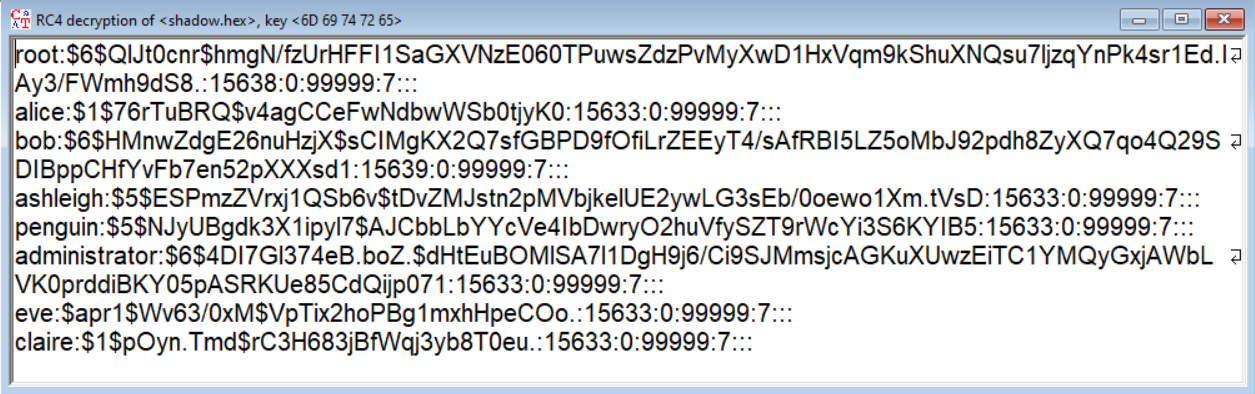
\includegraphics[width=0.85\columnwidth]{problem5/decryptshadow.PNG}
			}
		\caption{Content of the decrypted ``{\tt shadow.hex}'' file}
		\end{figure}
		
		
		
		\item Run ``John the Ripper'' password cracking utility to crack the passwords in the decrypted shadow file with the help of the dictionary ``rockyou.txt''(\href{https://uniofmora-my.sharepoint.com/:t:/g/personal/scharles_uom_lk/EQvMHge3CrZNpeE7WGXpapoBslFMMcgHih0teepNIwDVIg?e=9aEjJd}{Link}). What is the command you used to crack the passwords in the shadow file?\\		
		
		``\textit{Note that John can't crack hashes of different
			types at the same time.  If you happen to get a password file that has more than one hash type, you have to invoke John once for each hash type and you need to use this option to make John crack hashes of types other than the one it would auto-detect by default.}'' - abstracted from \href{https://github.com/openwall/john/blob/bleeding-jumbo/doc/OPTIONS}{here}.\\
		
		%% TODO: add answer here
		\begin{table}[!h]
			\centering
			\begin{tabular}{|c | l | l |}
				\hline
		\textbf{Hash ID} & \textbf{Hash format in John} & \textbf{Users}\\\hline
		{\tt \$6\$} & {\tt sha512crypt} & root, bob, administrator\\
		{\tt \$5\$} & {\tt sha256crypt} & ashleigh, penguin\\
		{\tt \$1\$, \$apr1\$} & {\tt md5crypt} & alice, eve, claire\\
		\hline\hline		
			\end{tabular}
		\caption{Additional {\tt --format} argument that should be passed to crack password}
		\end{table}
		
		\textbf{Note}:  ``{\tt resources}'' in the following command is a user created directory to keep the password list and the decrypted shadow file.\\
	
		Following commands were invoked one after the other to crack all the possible passwords in the given shadow file.\\
		
		{\footnotesize \tt \$ ./john --wordlist=resources/rockyou.txt --rules resources/Cry-RC4-shadow.txt --format=md5crypt}\\
		{\footnotesize \tt \$ ./john --wordlist=resources/rockyou.txt --rules resources/Cry-RC4-shadow.txt --format=sha256crypt}\\
		{\footnotesize \tt \$ ./john --wordlist=resources/rockyou.txt --rules resources/Cry-RC4-shadow.txt --format=sha512crypt}
		
		 \begin{figure}[H]
		 	\centering
		 	\fbox{
		 		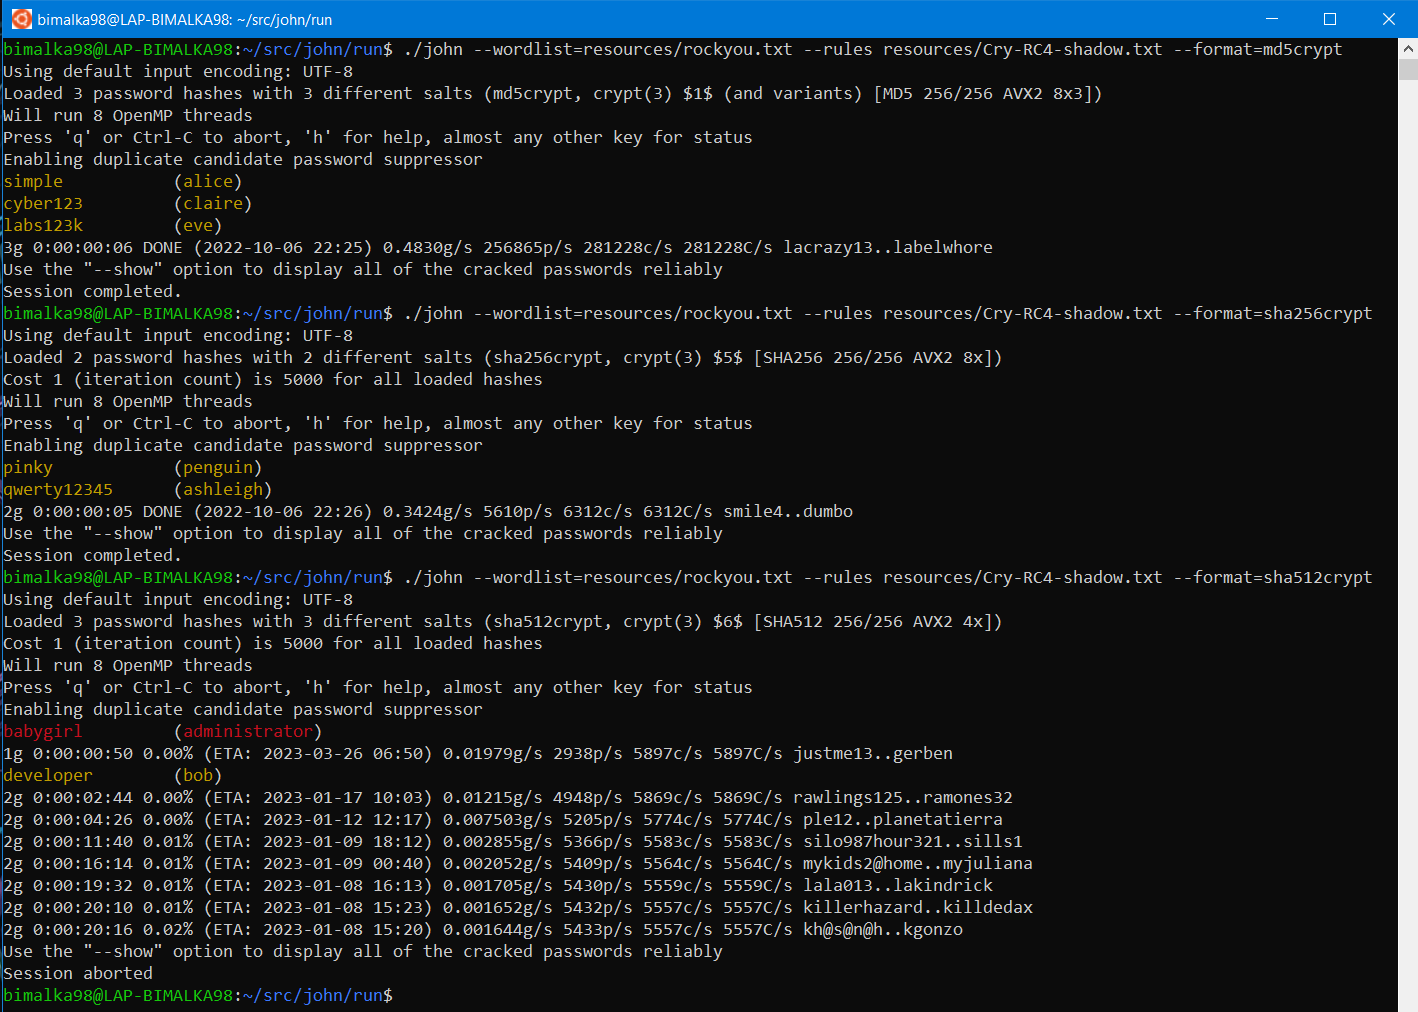
\includegraphics[width=0.85\columnwidth]{problem5/cracked.PNG}
		 	}
		 	\caption{Status of \textit{John the Ripper} while cracking the passwords }
		 \end{figure}
		
		It was observed that, the Estimated Time of Arrival(ETA) to crack the password of the \textit{root} user is 2023-01-XX and its progress increments really slowly. Therefore the program was aborted without trying to crack it.
		
		%%%%%%%%%%%%%%%%%%%%%
		%%%%%%%%%%%%%%%%%%%%%
		%%%%%%%%%%%%%%%%%%%%%
		
		\item Add a screenshot of all the cracked passwords.
		
		%% TODO: add answer here
		
		\begin{figure}[H]
			\centering
			\fbox{
				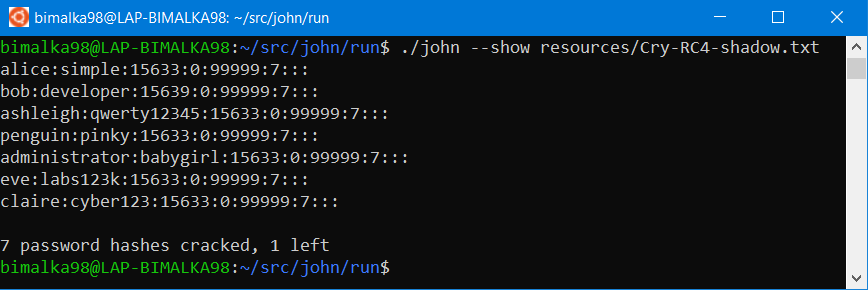
\includegraphics[width=0.85\columnwidth]{problem5/johnshow.PNG}
			}
			\caption{All the cracked passwords}
		\end{figure}
		\pagebreak
		\item Provide recommendations to enhance the strength of the passwords.
		
		By observing time duration the program took to crack each password, following recommendations can be provided.
		
		\begin{itemize}
			\item When creating a password a combination of numbers, letters (upper case and/or lower case)  and special characters must be used and the password must be sufficiently long to make it stronger.
			
			\item When selecting an encryption method, SHA-512 is preferred over SHA-256 and the MD5. Because the latter two methods were comparably weak and the passwords of the \textit{ashleigh, penguin, alice, eve} and \textit{claire} were cracked in less than 10 seconds. Whereas it took 50 seconds to guess the password of \textit{administrator} and nearly two minutes to crack the password of the \textit{bob}.
			
			\item When creating a password common words (such as \textit{simple, cyber,labs (found above)  and etc} ) and patterns (such as \textit{123, 12345 (found above) and etc} ) must be strictly avoided. As these words can be easily guessed and cracked in no time as seen in the above scenario.					
			
			\item A password must not contain personal information such as name, birth year and etc. as those can easily be combined to form a candidate set of passwords easily.
		\end{itemize}
		
		
		
		\clearpage
		
	\end{enumerate}    
	
	%%%%%%%%%%%%%%%%%%%%%%%%%%%%%%%%%
	%%%%%%%%%%%%%%%%%%%%%%%%%%%%%%%%%    
\end{document}
